\documentclass[11pt]{article}

\usepackage{sectsty}
\usepackage{graphicx}

% Margins
\topmargin=-0.45in
\evensidemargin=0in
\oddsidemargin=0in
\textwidth=6.5in
\textheight=9.0in
\headsep=0.25in

% Packages
\usepackage{indentfirst}
\usepackage{caption}

\title{A Small Tokamak for Education}
\author{Pavlo Vlastos}
\date{\today}

\begin{document}
	\maketitle	
	% Optional TOC
	% \tableofcontents
	% \pagebreak
	
	%--Paper--
	
	\section{Introduction}
	\indent This document outlines a project to build a small Tokamak. The intent is to make it easy to build and change to help reduce time for setting up experiments. The Tokamak is meant to hold plasma. The project focus is on building a strong understanding and intuition of the dynamics of a fully ionized gas in the presence of electromagnetic fields.
	
	\section{Design}
	[ADD CAD MODEL WITH DESCRIPTION]
	
	A copper coil is located in the center of a cylindrical chamber. The chamber holds a vacuum. A current is sent through the coil to make an electromagnetic field. The field lines are poloidal. A number of hydrogen atoms are injected into the chamber. The electrons are stripped from their respective protons; their energy levels are increased. [How?] The resulting ions ``fly'' around the the coil, following the electromagnetic field lines. 
	
	\subsection{Adjust-ability}
	The design of the Tokamak will be made adjustable. The idea is to make it easy to set up different experiments without having to machine many new parts.
	
	\section{Design Questions}
	\subsection{Coils}
	\begin{enumerate}
		\item How many polodial and torodial coils are necessary for stable plasma confinement?
		\item How many turns for each (set of) coils (including the central solenoid)?
		\item What is the optimal placement of the coils?
	\end{enumerate}

	\section{System Design}
	\begin{figure}[hbt!]
		\centering
		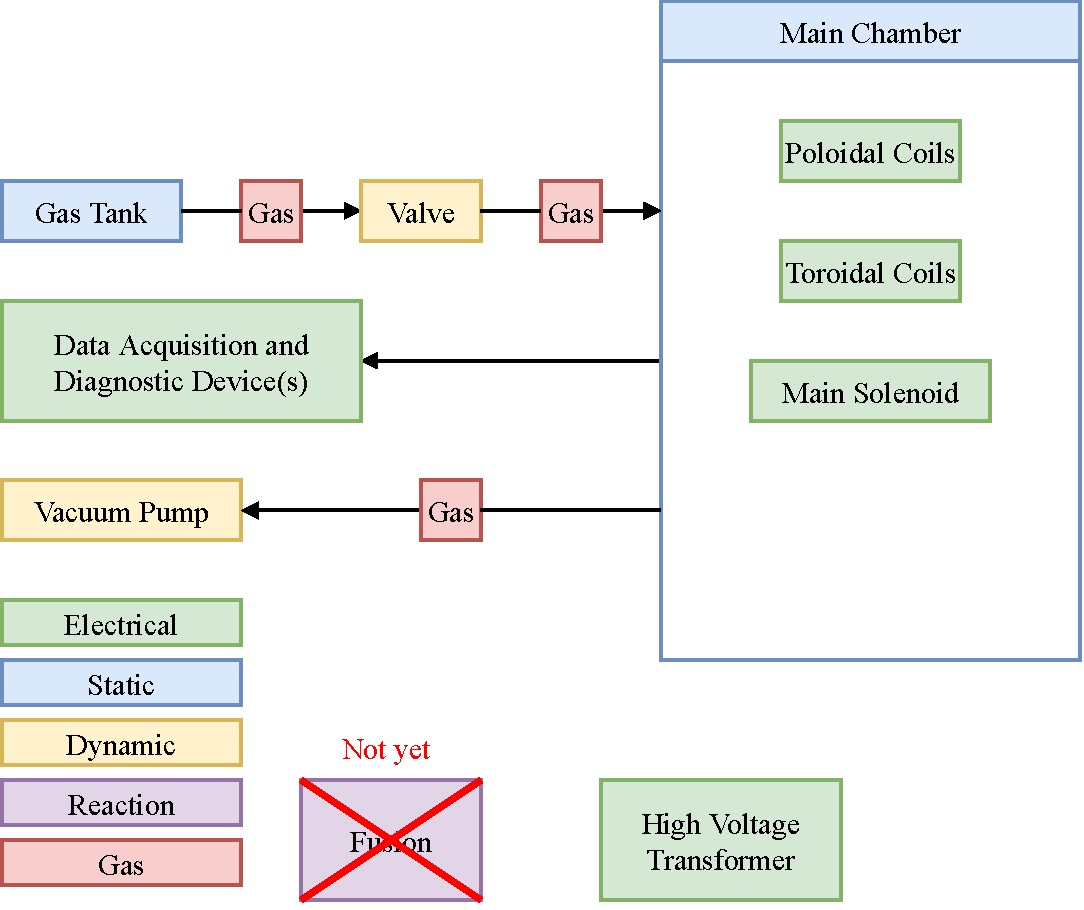
\includegraphics[width=0.75\textwidth]{images/F001_system_block_diagram.pdf}
		\captionsetup{width=\textwidth}
		\caption{The living system block diagram for the F001 Tokamak.}
		\label{fig:F001_system_block_diagram}
	\end{figure}
	
	%--/Paper--
	
\end{document}